\subsection{Experimental Results}\label{subsec:experimental-results}

\subsubsection{Input Workpiece Variation}\label{subsubsec:input-workpiece-variation}

\subsubsection{Pause Duration Variation}\label{subsubsec:pause-duration-variation}

\begin{figure}
    \centering
    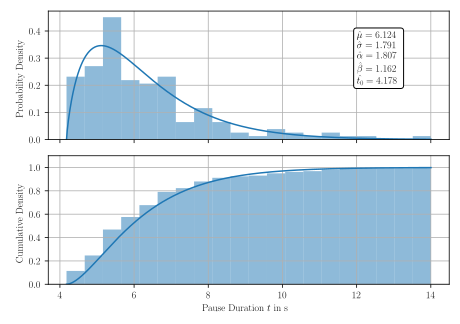
\includegraphics[width=\linewidth]{img/plot_histogram_pauses}
    \caption{Density and Cumulative Histograms of Inter-Pass Durations With Fitted Gamma Distribution}
    \label{fig:plot_histogram_pauses}
\end{figure}


\subsection{Simulation Results}\label{subsec:simulation-results}

In the following, three questions shall be investigated and answered:
\begin{enumerate}
    \item What is the difference in behavior of variations sourced in the input workpiece and arising within the process?
    \item What is the influence of elastic mill response on the variational behavior of the process?
    \item Is there a minimum number of passes needed to eliminate variations of the input workpiece?
\end{enumerate}

For this distinct simulations were carried out and compared with each other and the experimental data.

\subsubsection{Different Sources of Variation}\label{subsubsec:different-sources-of-variation}

\subsubsection{Influence of Elastic Mill Response}\label{subsubsec:influence-of-elastic-mill-response}

\subsubsection{Elimination of Input Variation}\label{subsubsec:elimination-of-input-variation}